%!TEX root = main_arduino_intro.tex

\chapter{Thermoelectric cooling element}\label{chap:tec}

The final part that we need to implement in order to build a sample cooling system is the actual cooling element. As a cooling element, we will use a Peltier cooler from \href{https://www.adafruit.com/product/1335}{Adafruit}, which is mounted onto a heat sink and fan assembly.


\section{Components and their Physics}

\subsection{The Peltier effect}\label{sec:tec:peltier_effect}

Thermoelectric coolers make use of the so-called Peltier effect in order to create a heat flux between two different types of materials. This means that heat flows from one element to the other, i.e., that one side gets cold and the other one hot. The Peltier effect was discovered in 1834 by French Physicist \href{https://en.wikipedia.org/wiki/Jean_Charles_Athanase_Peltier}{Jean Charles Athanase Peltier}. In principle, it works similar to a thermocouple, which we discussed above.
\begin{figure}[b!]
    \centering
    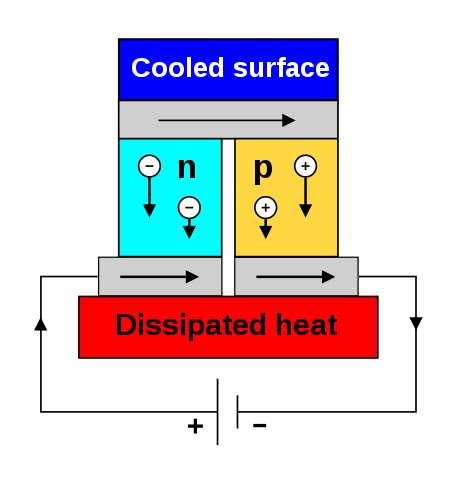
\includegraphics[width=0.35\textwidth]{graphics/04_peltier/peltier_cooler}
    \caption{The Peltier effect acting on a thermoelectric cooler. Credit: \href{https://en.wikipedia.org/wiki/File:Thermoelectric_Cooler_Diagram.svg}{Ken Brazier via Wikipedia}, License: \href{https://creativecommons.org/licenses/by-sa/4.0/}{CC BY-SA 4.0}}
    \label{fig:peltier:peltier}
\end{figure}
Figure~\ref{fig:peltier:peltier} shows a schematic on how the Peltier effect is used to create a thermoelectric cooler. Here, an n- and a p-doped semiconductor are brought together. If we simply measure the voltage across the two metals, we can use the setup as a thermocouple. (Note that this is different from a thermistor, see introduction to Chapter~\ref{chap:temperature}.) If we power the setup with a \ac{dc} voltage, a heat flow is generated. The heat flow per unit time is given as
\begin{equation}
    \dot{Q} = (\Pi_m - \Pi_n)I.
\end{equation}
Here, $\Pi_m$ and $\Pi_n$ are the Peltier coefficients of the two semiconductors and $I$ is the current. Not that the amount of heat flow is directly proportional to the current.

A typical thermoelectric cooler contains many semiconductor junctions added together in series. Furthermore, in order to achieve efficient cooling on one side, the heat from the hot side needs to be removed. This is generally done by mounting the hot side on a heat sink. In our case, the heat sink is connected to a fan which helps to remove heat faster.


\subsection{\acs{mosfet}}

The Peltier cooler that we will be using draws 5\,A of current at 12\,V. The voltage and especially the current are too high for any Arduino pin. We therefore need to implement a switch that we can turn on and off via an Arduino pin and that can handle high currents in order to drive the cooling element. One type of switch that can drive our circuit is a \acf{mosfet}.

\qbox{One issue of driving the cooler directly from the Arduino is the that the pins only put out 5\,V. At this voltage, what current would be drawn by the Peltier cooler? Compare this current with the maximum current that an Arduino pin can supply. What would happen if you try to drive the cooler off a 5\,V pin?}

 \begin{figure}[bt]
     \centering
     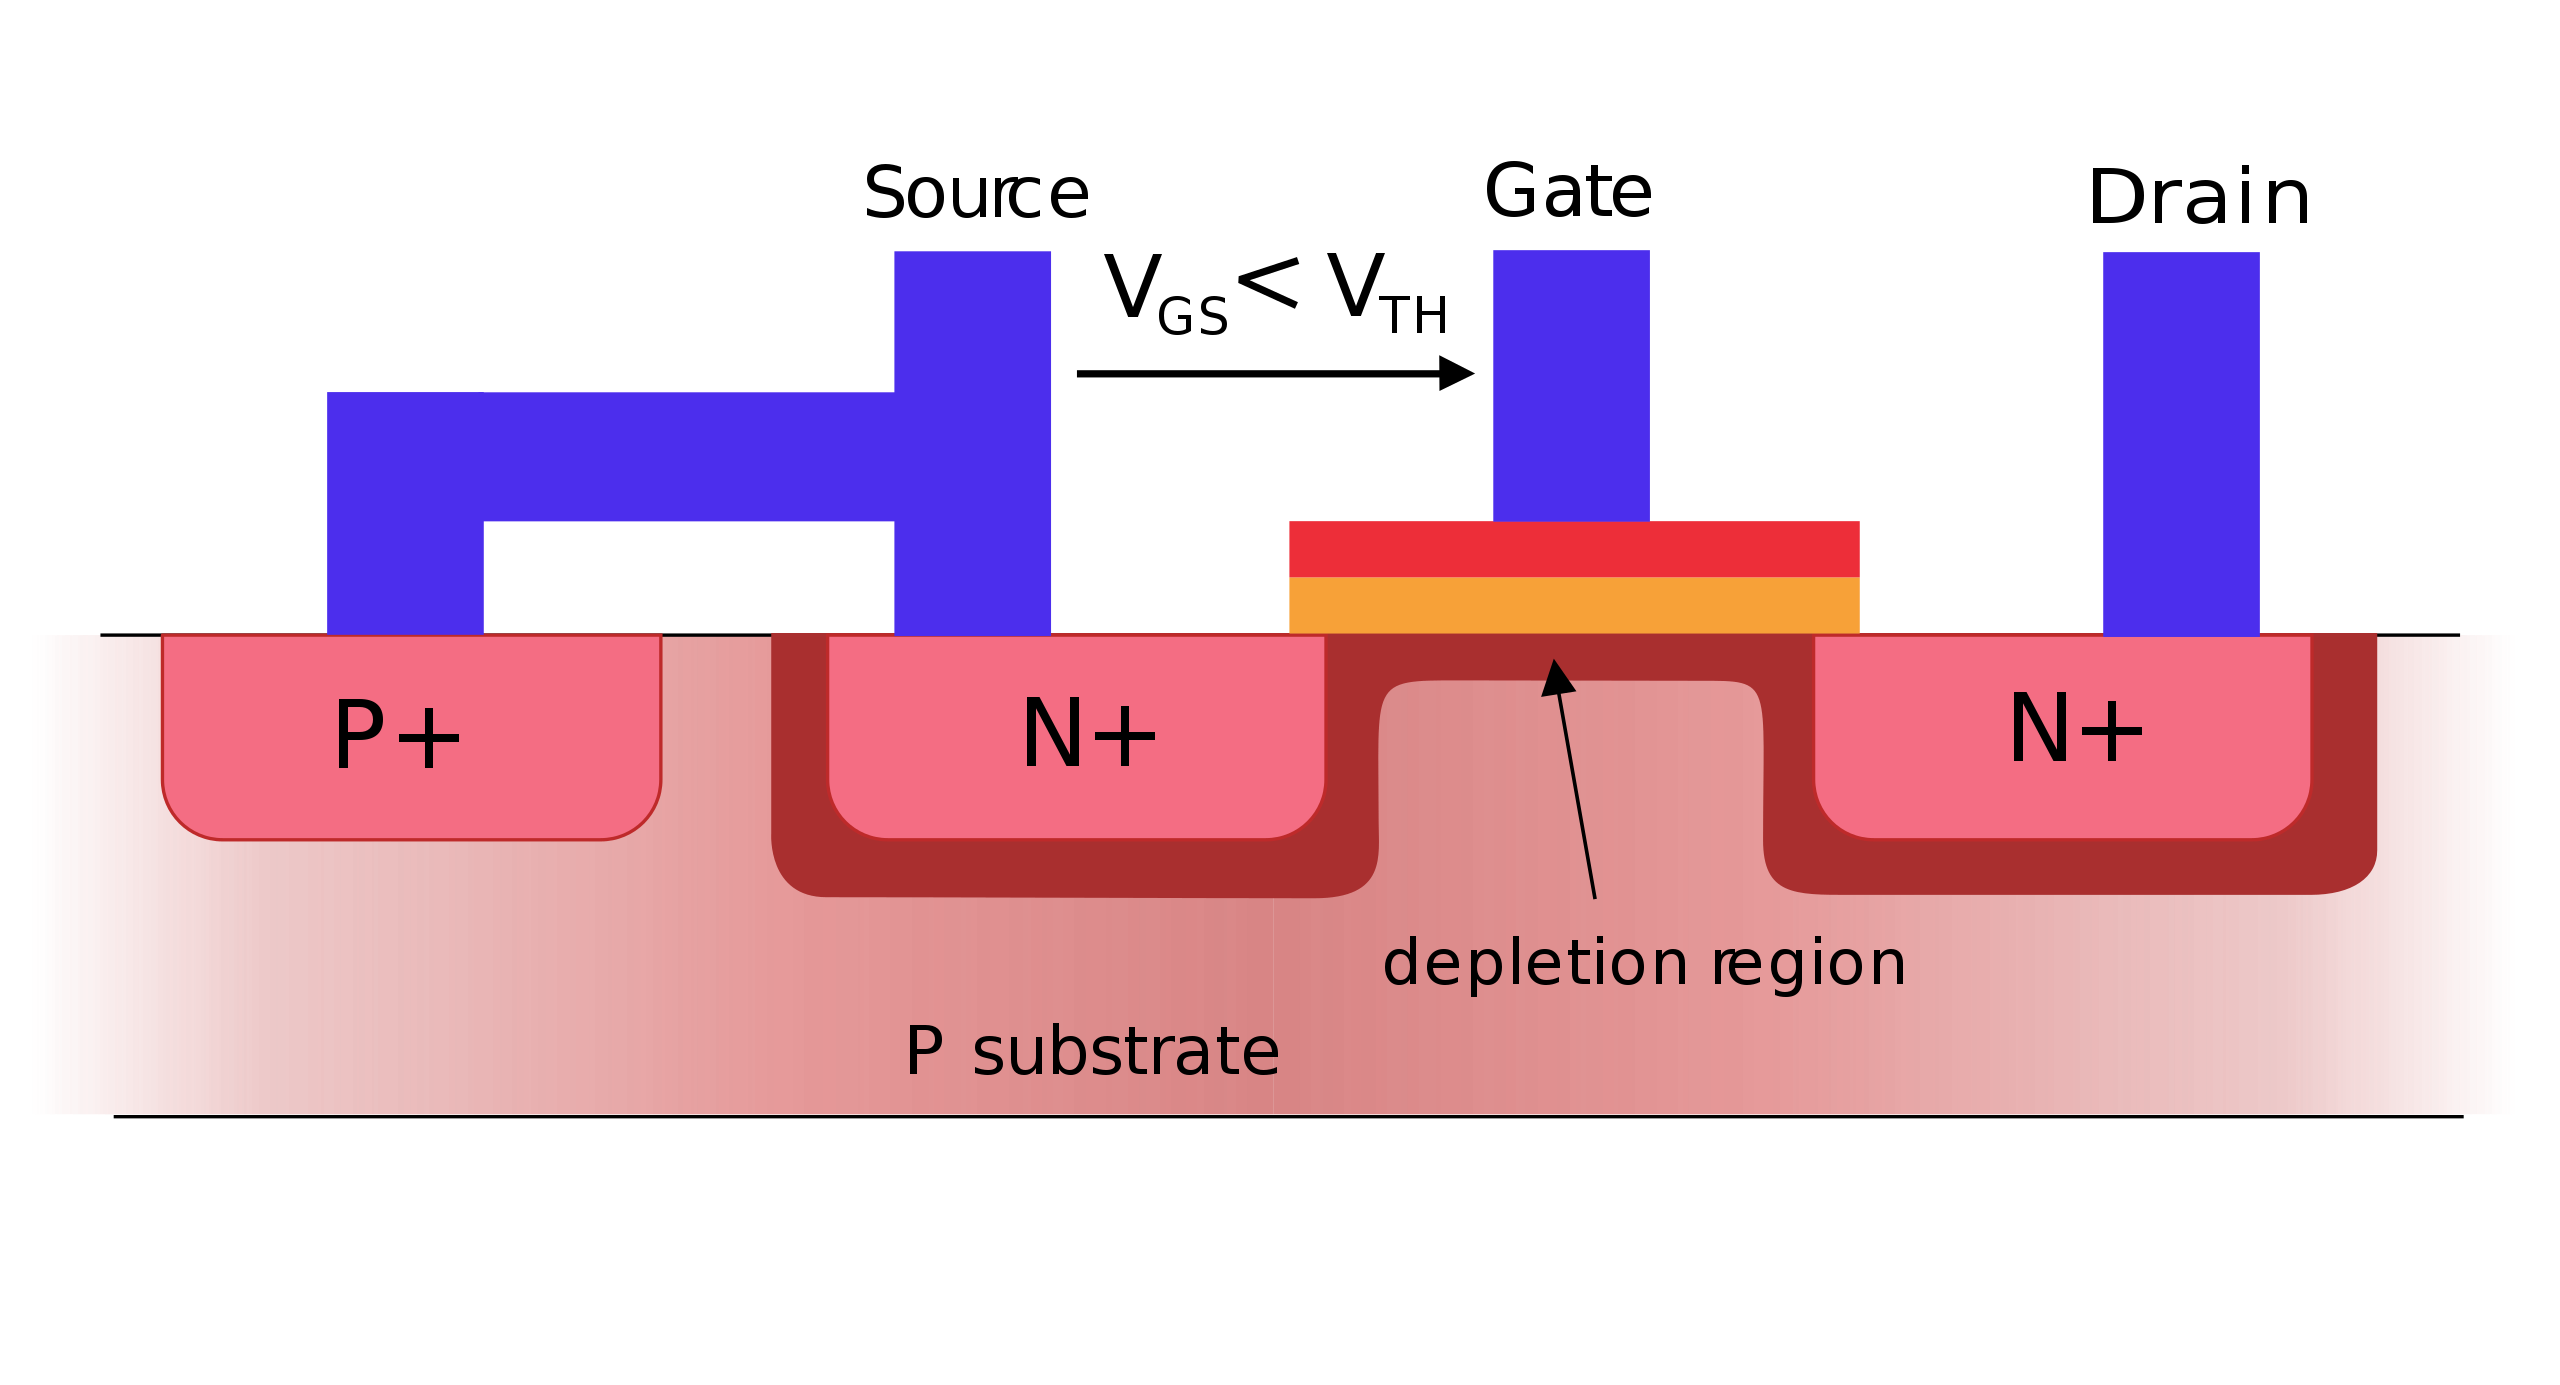
\includegraphics[width=0.6\textwidth]{graphics/04_peltier/nMOSFET.png}
     \caption{A cross-section through an n\ac{mosfet}. See text for a detailed description. Credit: \href{https://en.wikipedia.org/wiki/MOSFET\#/media/File:MOSFET_functioning_body.svg}{Wikipedia}, License: \href{https://creativecommons.org/licenses/by-sa/3.0/}{CC BY-SA 3.0}.}
     \label{fig:peltier:nmosfet}
 \end{figure}
 \Acp{mosfet} are ideal devices to use as high-current switches that can be rapidly turned on and off by simply using an Arduino pin.
Figure~\ref{fig:peltier:nmosfet} shows the inner workings of an n-type \ac{mosfet}, also often referred to as an NMOS. The source and drain on an n\ac{mosfet} are n-type materials, i.e., they contain a surplus of electrons and are therefore electron donors. These two channels are inside a p-type substrate which lacks electrons and is therefore an electron acceptor. When simply applying a voltage in between source and drain, the p-type material in between does not allow a current to flow. However, by applying a positive voltage to the gate, electrons are attracted to the gate area, which creates a conductive band allowing current to flow in between the source and the drain.

\Acp{mosfet} can have wildly different specifications. For Arduino electronics, we want to utilize the ones for which the gate switches when applying a low voltage of only 5\,V. Furthermore, we need a \ac{mosfet} that can at least handle 5\,A of current. At high currents, \acp{mosfet} can get hot and might need to be mounted to a cooling element themselves. In our case however, the \ac{mosfet} can be air-cooled up to a current of $\sim$15\,A, therefore, a cooling element will not be necessary at the 5\,A used here.

Since \acp{mosfet} allow for rapid switching, they can also be driven from \ac{pwm} pins. This allows you to regulate the current to the cooler and therefore to cool it more and less efficiently.

\morebox{Some applications for \acp{mosfet}}{Using \acp{mosfet} allows you to rapidly switch various voltages and work with high currents. Furthermore, the high-frequency switching allows you to control the current by connecting the gate to a \ac{pwm} pin. For example, \acp{mosfet} are frequently used as motor drivers. In order to have a motor run backwards it is often required to have a setup that can switch polarities. To enable this, an \href{https://en.wikipedia.org/wiki/H-bridge}{H-bridge} can be used.}


\section{Implementing a \ac{mosfet} controlled Peltier cooler}

\begin{figure}[bt]
    \centering
    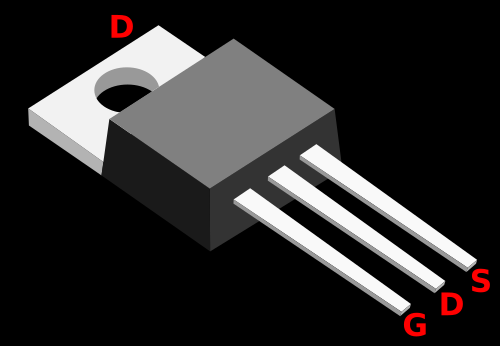
\includegraphics[height=3cm]{graphics/04_peltier/nmos_pins.png}\hspace{2cm}
    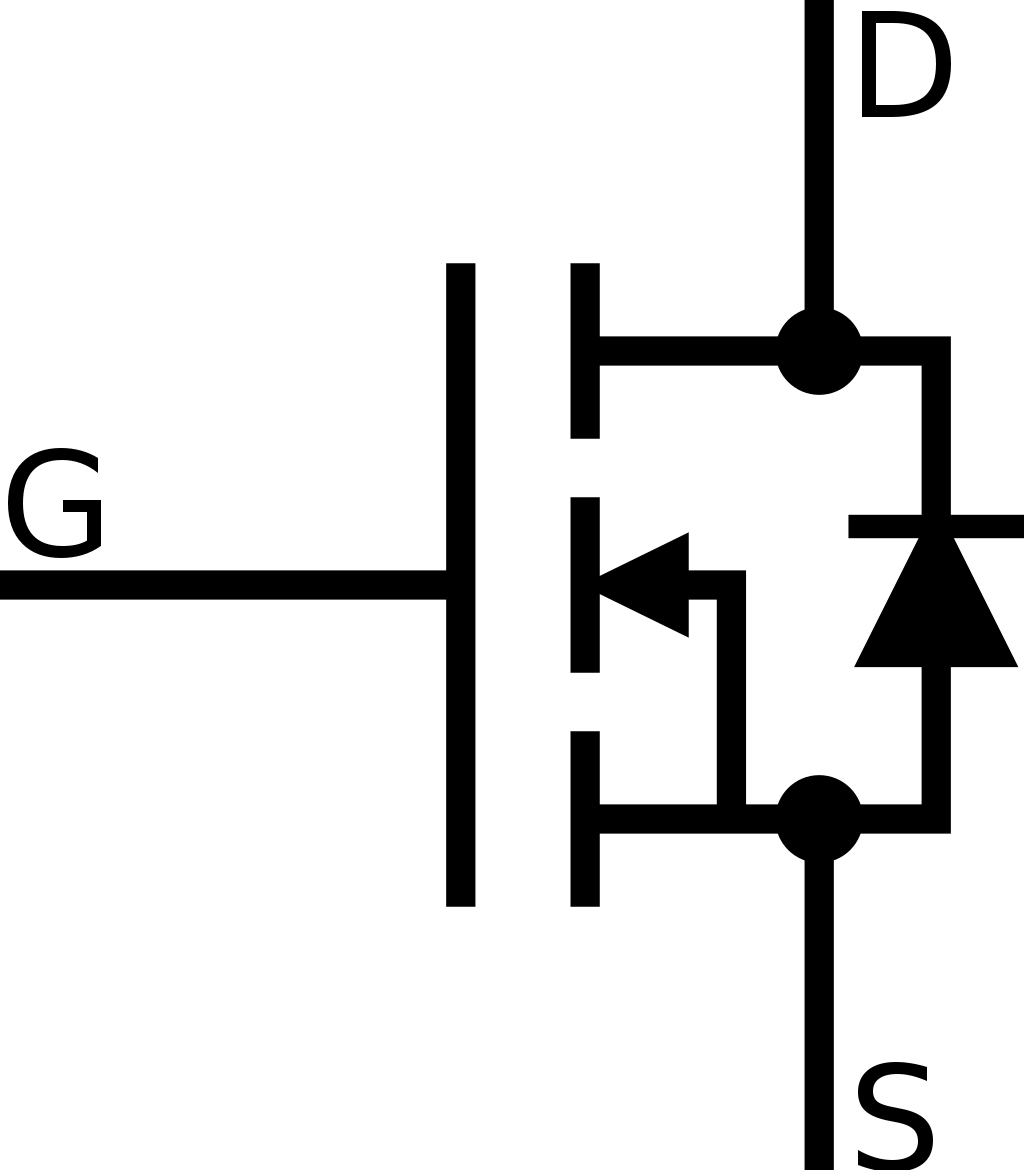
\includegraphics[height=3cm]{graphics/04_peltier/nMOSFET_symbol.png}
    \caption{Schematic with pin assignments of the n\ac{mosfet} we are using here (left) and electrical symbol of a n\ac{mosfet} (right). Note the diode connecting the source (S) to the drain (D). The gate is labeled G. (Right image credit: \href{https://en.wikipedia.org/wiki/Electronic_symbol\#/media/File:Enh_N_channel_Mosfet.svg}{ErikBuer via Wikipedia}, license: \href{https://creativecommons.org/licenses/by-sa/4.0/}{CC BY-SA 4.0}.)}
    \label{fig:peltier:mosfet_used}
\end{figure}
Figure~\ref{fig:peltier:mosfet_used} shows a schematic (left) and the electrical symbol (right) of the n\ac{mosfet} that we are using here. The data sheet can be found \href{https://cdn-shop.adafruit.com/datasheets/irlb8721pbf.pdf}{here}. As shown in the electrical symbol, this n\ac{mosfet} has an additional diode in between the source and the drain. This means that current can flow between the source and then drain even when we do not apply a gate voltage. For the n\ac{mosfet} to actually work as a switch, we need to set it up such that, when switched, the current flows from the drain to the source. 

\qbox{With above mentioned considerations in mind, draw a circuit diagram that allows you to control the 12\,V power supply to drive the thermoelectric cooler from a 5\,V Arduino pin. In which part of your circuit diagram will the full 5\,A current flow when the gate is activated? Make sure that the 5\,V from the gate is connected to ground via a 10\,k$\Omega$ resistor, such that it is not floating when turned off (remember that an Arduino \ac{io} pin configured as an ouptut cannot be used as a voltage sink). Also make sure that the 12\,V power supply and your Arduino share a common ground! If no common ground is established, the gate will be floating, which could damage the \ac{mosfet} by overheating it.}

If you are having trouble with this exercise, a mock setup can be found on \href{https://www.tinkercad.com/things/559YKkQD8tB}{TinkerCAD}. The thermoelectric cooler is here represented by a 2.4\,$\Omega$ resistor. If you run the simulation, it will slowly increase the voltage every three seconds. The voltage and current applied to the ``cooler'' are displayed on a volt and ampere meter, respectively.

\exerbox{Now implement the above wiring diagram in real life. Before you connect the 12\,V to the actual power supply, make sure that:
\begin{itemize}
    \item You did not connect 12\,V to any Arduino \ac{io} pins
    \item The full 5\,A current does not flow through the breadboard at any point
\end{itemize}
Double check this carefuflly since, if not connected properly, you might destroy the Arduino and / or the breadboard. Also connect the fan of the thermoelectric cooler to the 12\,V, however, connect it such that it is permanently on when the 12\,V are connected.}

As mentioned above, the breadboard cannot handle 5\,A of current since the leads are too small. Small wires have a higher resistance per unit length compared to wires with larger diameters and therefore get hotter when a given amount of current flows through them. We thus have to use appropriate wiring. In the US, wire sizes are standardized and given in units of \ac{awg}. The lower the number in \ac{awg}, the thicker is the wire we are dealing with. Tables such as \href{https://en.wikipedia.org/wiki/American_wire_gauge}{these ones} show how much current can be carried by any given wire. As you can see, a 20\,\ac{awg} wire can carry 5\,A and would therefore be sufficient to be used for the Peltier cooler.

\exerbox{Turn on the thermoelectric cooler with different \ac{pwm} outputs on the gate and verify (1) that the cooler actually gets cold and (2) that the voltage applied across the cooler is what you would expect from your \ac{pwm} output level. Control the cooler from a subroutine that allows you to easily set the power level from the main loop.}

\exerbox{Using Kapton tape, stick the thermistor on the surface of the thermoelectric cooler. First measure the room temperature and then the lowest temperature that the Peltier element can reach for varying control levels. To record the temperature you can either display it on the seven-segment display or print it out via serial.}

\exerbox{Now that you have an idea on how cool the Peltier element can get, set it to maximum cooling and turn off the cooling fan. What happens to the temperature and why?}
